\chapter{Reference Algorithm} \label{Algorithm}

The contents of this chapter are informative only.

A reference algorithm for compressed branch trace is given in figure~\ref{fig:algo}.  
In the diagram, the following terms are used:

\begin{itemize}
  \item \textit{te\_inst.} The name of the packet type emitted by the encoder (see Chapter~\ref{packets});
  \item \textit{inst.}  Abbreviation for 'instruction';
  \item \textit{updiscon.}  Uninferable PC discontinuity.  This identifies an instruction that
    causes the program counter to be changed by an amount that cannot be predicted from the
    source code alone (\textbf{itype} values 8, 10, 12 or 14);
  \item \textit{Qualified?}  An instruction that meets the filtering criteria is qualified, and will be traced;
  \item \textit{Branch?} Is the instruction a branch or not (\textbf{itype} values 4 or 5);
  \item \textit{branch map.}  A vector where each bit represents the outcome of a branch.  A 0 indicates the
    branch was taken, a 1 indicates that it was not;
  \item \textit{e\_ccd.} An exception has been signalled, or context has changed and
    should be treated as an uninferable PC discontinuity (see Table~\ref{tab:context-type});
  \item \textit{ppch.} Privilege has changed, or context has changed and needs to be 
    reported precisely (see Table~\ref{tab:context-type});
  \item \textit{ppch\_br.} As above, but branch map not empty;
  \item \textit{er\_ccdn.}  Instruction retirement and exception signalled on the same cycle, 
    or context has changed and should be treated as an uninferable PC discontinuity, or
    context notification (see Table~\ref{tab:context-type});
  \item \textit{exc\_only.}  Exception signalled without simultaneous retirement;
  \item \textit{cci.}  context change that can be reported imprecisely (see Table~\ref{tab:context-type});
  \item \textit{rep\_br.} Report branches due to full branch map or misprediction;
  \item \textit{branches.}  The number of branches encountered but not yet reported to the decoder;
  \item \textit{pbc.} Correctly predicted branches count (always zero if branch predictor disabled or not present);
  \item \textit{resync count.} A counter used to keep track of when it is necessary to send 
    a synchronization packet (see Section~\ref{sec:resync});
  \item \textit{max\_resync.}  The resync counter value that schedules a synchronization packet (see Section~\ref{sec:resync});
  \item \textit{resync\_br.} The resync counter has reached the maximum value and there are
    entries in the branch map that have not yet been output (see Section~\ref{sec:resync}).
\end{itemize}

\begin{figure}
\begin{center}
  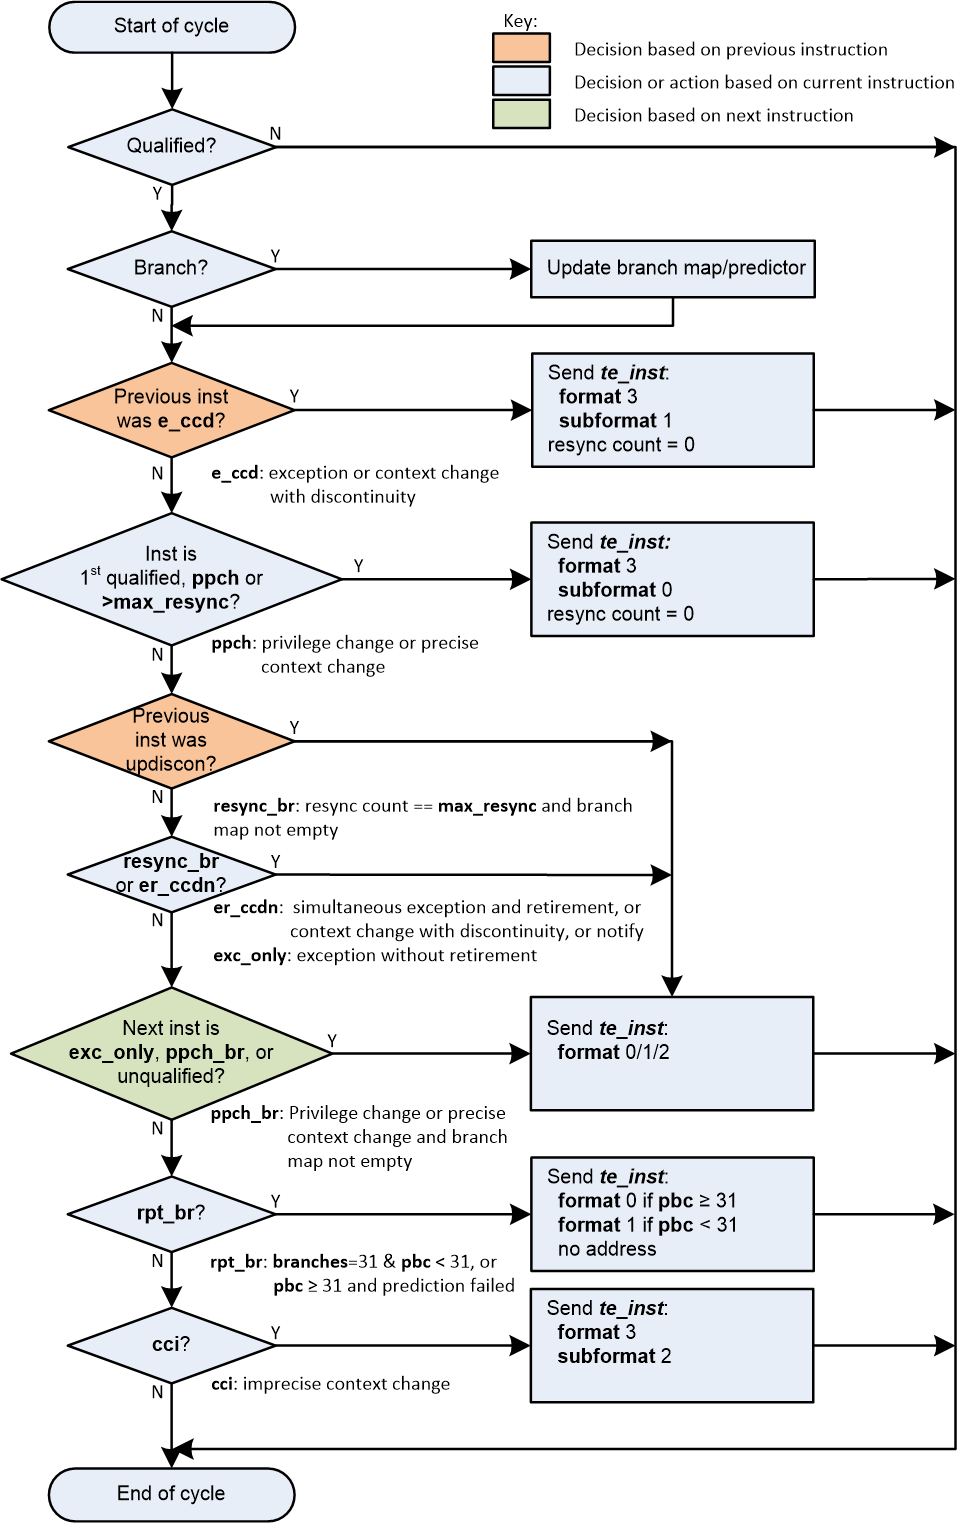
\includegraphics[height=23cm, width=15cm]{algo.png}
  \caption{Instruction delta trace algorithm}
  \label{fig:algo}
\end{center}
\end{figure}

Figure~\ref{fig:algo} shows instruction by instruction behavior, as would be
seen in a single-retirement system only.  Whilst the core to encoder interface allows the 
RISC-V hart to provide information on multiple retiring instructions simultaneously, the resultant 
packet sequence generated by the encoder must be the same as if retiring one instruction at a time.

A 3-stage pipeline within the encoder is assumed, such that the encoder has 
visibility of the current, previous and next instructions.  All packets are generated using 
information relating to the current instruction.  The orange diamonds indicate decisions 
based on the previous instruction, the green diamond indicates a decision based on the
next instruction, and all other diamonds are based on the current instruction.

Additionally, the encoder can generate one further packet type, not shown on the diagram for 
clarity.  The \textit{support} packet (format 3, subformat 3 - see section~\ref{sec:format33}) is 
sent when:

\begin{itemize}
  \item The encoder is enabled or disabled, or its configuration is changed, 
    to inform the decoder of the operating mode of the encoder;
  \item After the final qualified instruction has been traced, to inform the decoder that 
    tracing has stopped;
  \item If trace packets are lost (for example if the buffer into which packets are being 
    written fills up.  In this situation, the 1st packet 
    loaded into the buffer when space next becomes available must be a \textit{support} 
    packet.  Following this, tracing will resume with a sync packet.
\end{itemize}

Note: if the \textbf{halted} or \textbf{reset} sideband signals are asserted (see Table~\ref{tab:ingress-side-band})
the encoder will behave as if it has received an unqualified instruction (output \textit{te\_inst}
reporting the address of the previous instruction, followed by \textit{te\_support});


\section{Format selection} \label{format-selection}

In all cases but two, the packet format is determined only by a 'yes' outcome from the 
associated decision.  

When reporting branch information on its own (without an address), the choice between format 1 and format 0, 
subformat 0 depends on the number of correctly predicted branches (this will be 0 if the predictor is not 
supported, or is disabled).  No packets are generated until there are at least 31 branches to report.  
Format 1 is used if the outcome of at least one of those 31 branches was not predicted correctly.  If all were 
predicted correctly, nothing is output at this time, and the encoder continues to count correctly predicted
branch outcomes.  As soon as one of the branch outcomes is not correctly predicted, the encoder will output
a format 0, subformat 0 packet.  See also section~\ref{sec:format0}.

The choice between formats 0, 1 or 2 for the case in the middle of the diagram annotated "address always included"
also needs further explanation.  

\begin{itemize}
  \item If the number of correctly predicted branches is 31 or more, then format 0, subformat 0 is
    always used;
  \item Else, if the jump target cache is supported and enabled, and the address being reported is in the cache,
    then normally format 0, subformat 1 will be used, reporting the cache index associated with the address.  
    This will include branch information if there are any branches to report.  
    However, the encoder may chose to output the equivalent format 1 or 2 packet (containing the differential 
    address, with or without branch information) if that will result in a shorter packet 
    (see section~\ref{sec:format0});
  \item Else, if there are branches to report, format 1 is used, otherwise format 2.
\end{itemize}


Packet formats 0, 1 and 2 are organized so that the address is usually the final field.  Minimizing the 
number of bits required to represent the address reduces the total packet size and significantly
improves efficiency.  See Chapter~\ref{packets}.

\section{Resynchronisation} \label{sec:resync}

Per Section~\ref{synchronization}, a format 3 synchronisation packet must be output after "a prolonged
period of time". The exact mechanism for
determining this is not specified, but options might be to count the number of \textit{te\_inst} packets emitted, 
or the number of clock cycles elapsed, since the previous synchronization message was sent.

When the resync is required, the primary objective is to output a format 3 packet, so that the decoder can 
start tracing from that point without needing any of the history.  However, if the decoder is already synced, 
then it is also required that it can continue to follow the execution path up to and through the format 3 packet 
seamlessly.  As such, before outputting a format 3 packet, it is necessary to output a format 1 packet for the 
preceding instruction if there are any unreported branches (because format 3 does not contain a branch map).  
The format 3 will be sent if the resync timer has been exceeded.  On the cycle before this (when the resync timer 
value has been exactly reached), a format 1 will be generated if the branch map is not empty.

\section{Multiple retirement considerations} \label{rec:multiretcon}

As noted earlier in this section, for a single-retirement system the reference algorithm is applied to each retired
instruction.  When instructions are retired in blocks, only the first and last instruction in a block need be
considered, as all those in between are "uninteresting", and will have no effect on the encoder's state (their route
through figure~\ref{fig:algo} does not pass through any of the rectangular boxes).

In most cases, either the first or last instruction of a block (but not both) is interesting, meaning that the 
encoder does not need to generate more than one packet from a block.  However, there are a few cases where this
is not true, and it is possible that the encoder will need to generate two packets from the same block.  

For example, the first instruction in a block must generate a packet if it is the first traced instruction.  However,
if the block also indicates an exception or interrupt (\textbf{itype}= 1 or 2), then the last instruction in the block 
must also generate a packet.

As generating multiple packets per cycle would significatly complicate the encoder, and as situations such as this
will only occur infrequently, some elastic buffering in the encoder is the preferred approach.  This will allow subsequent
blocks to be queued whilst the encoder generates two successive packets from a block.  The encoder can drain the 
elastic buffer any time there is a cycle when the hart doesn't report anything, or if there is a block with 
\textbf{itype} = 0 (which is uninteresting to the encoder).

There are pathological cases where consecutive blocks could require packets to be generated from both first and last
instructions, but elastic buffering is only required if the blocks are also input on consecutive cycles.  In practice
there are very few cases where this can occur.  The worst so far identified case is a variation on the example above, 
where the exception is an ecall, and that in turn encounters some other form of exception or interrupt in the first 
few instructions of the trap handler:

\begin{itemize}
  \item Block 1: \textbf{itype} = 1 (ecall), \textbf{iretires} > 1.  Generate packet from first instruction (first traced),
    and last instruction (last before ecall);
  \item Block 2: \textbf{itype} = 1 or 2 (some other exception or interrupt), \textbf{iretires} > 0.  
    Generate packet from first instruction (ecall trap handler), and last instruction (last before other exception or interrupt);
  \item Block 3: Generate packet from first instruction (other exception or interrupt trap handler)
\end{itemize}

Because the ecall is known to the hart's fetch unit and can be predicted, it may be possible for block 2 to occur the cycle 
after block 1.  However, it is reasonable to assume that the other exception or interrupt will not be predicatable, and as a result
there will be several cycles between blocks 2 and 3, which will allow the encoder to 'catch up'.  It is recommended that encoders
implement sufficient elastic buffering to handle this case, and if for some reason the elastic buffer overflows, it should
issue a support packet indicating trace lost.
